\section{Evaluierung der Methoden}
\label{sec:5}
\markboth{Evaluierung der Methoden}{Evaluierung der Methoden}

Beide Methoden haben ihre Vor- und Nachteile. Die realistische Darstellung von voluminösen Materialien verlangt
eine besondere Herangehensweise, welche sich – im Gegensatz zu undurchsichtigen, festen Oberflächen –
nicht überzeugend mit herkömmlichen Texture-Mapping Methoden umsetzen lässt.
Die Implementierung der Systeme ist aufgrund der begrenzten Zeit im Rahmen dieser Arbeit nur prototypisch mithilfe der
zur Verfügung stehenden Funktionen aus Unity implementiert und daher nicht bestmöglich optimiert.
In \textbf{\autoref{sec:6.3}} werden einige Optimierungsmöglichkeiten präsentiert.
Die Vor- und Nachteile, sowie das Potential für den Nutzen der jeweiligen Methoden lassen sich dennoch aus dem Entwurf
herausarbeiten und werden in den folgenden Abschnitten beschrieben.


\subsection{Parallax Occlusion Mapping}
\label{sec:5.1}


POM ist eine komplexere Variante des Normalmappings. Dementsprechend ist auch POM eine Technik für feste Oberflächen und weniger
für den Einsatz bei der Simulation von Volumen gedacht. Um aber die Effizienz der Billboard-basierten Partikelsysteme
nutzen zu können ist das Parallax Occlusion Mapping eine interessante Möglichkeit, die es wert ist, getestet zu werden.
Trotz der erhöhten Komplexität des Algorithmus gegenüber klassischeren Mappingverfahren läuft die Anwendung auf dem Testsystem
stabil mit 90FPS. Hier gibt es also keine Bedenken hinsichtlich der Shaderperformance. Auch die aufwändige Berechnung der
Fluidsimulationen wird hier im Voraus erledigt. Somit ist es möglich, realistisch aussehende Partikelsysteme unter geringem
Rechenaufwand in der Echtzeitanwendung zu erzeugen und diese dabei noch realistisch aussehen zu lassen.
Ein weiterer Vorteil, der sich aus der Natur des schwarzen Rauches bei Bränden ergibt, ist die Tatsache, dass die genaue Berechnung
von Selbstschattierungen hierbei nicht so essentiell ist wie bei weißem Rauch.
Dies ist zwar nicht direkt ein Vorteil von POM, gleicht aber einen Nachteil aus, den es in der Anwendung in einem Partikelsystem gibt.
Die Texturen auf den Billboards sind in der Lage, sich individuell selbst zu schattieren, gegenseitig ist dies jedoch nicht möglich (\textbf{\autoref{fig:pomShadows}}). 
In Bezug auf den Schatten generell gibt es das Problem, dass Billboard-basierte Partikelsysteme eigentlich nur flache Sprites sind und deshalb nicht in der 
Lage sind, realistische Schatten auf die Umgebung werfen zu können. In Hinblick auf die Beleuchtung ist es mit POM auch möglich, eine geringe Anzahl dynamischer 
Lichtquellen einzubeziehen (\textbf{\autoref{fig:dynamicLightingSmoke}}).

\begin{figure}[h!]
	\centering
	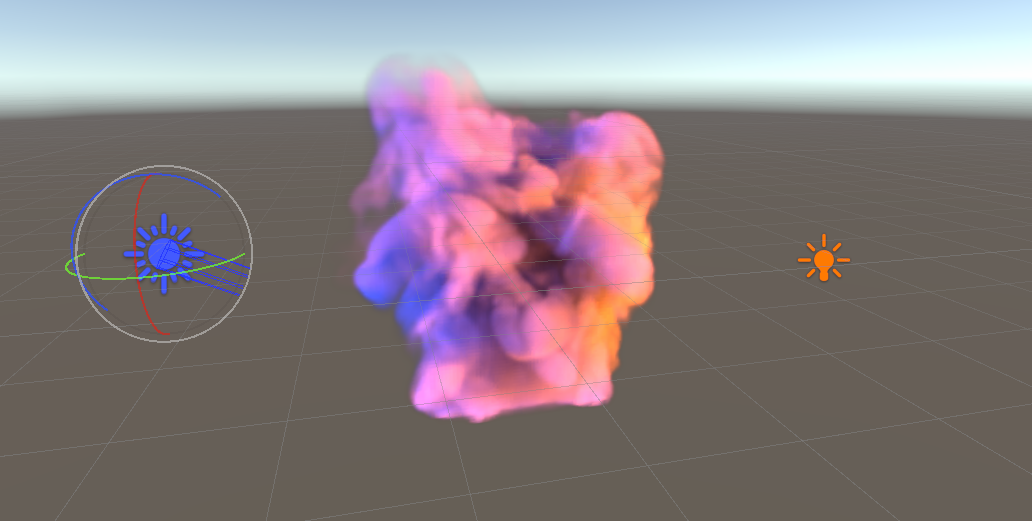
\includegraphics[width=0.89\textwidth]{Grafiken/Implementation/litSmoke.png}
	\begin{footnotesize}
		\caption{Dynamische Beleuchtung des Rauchs}
		\label{fig:dynamicLightingSmoke}
	\end{footnotesize}
\end{figure}



\begin{figure}[h!]
	\centering
	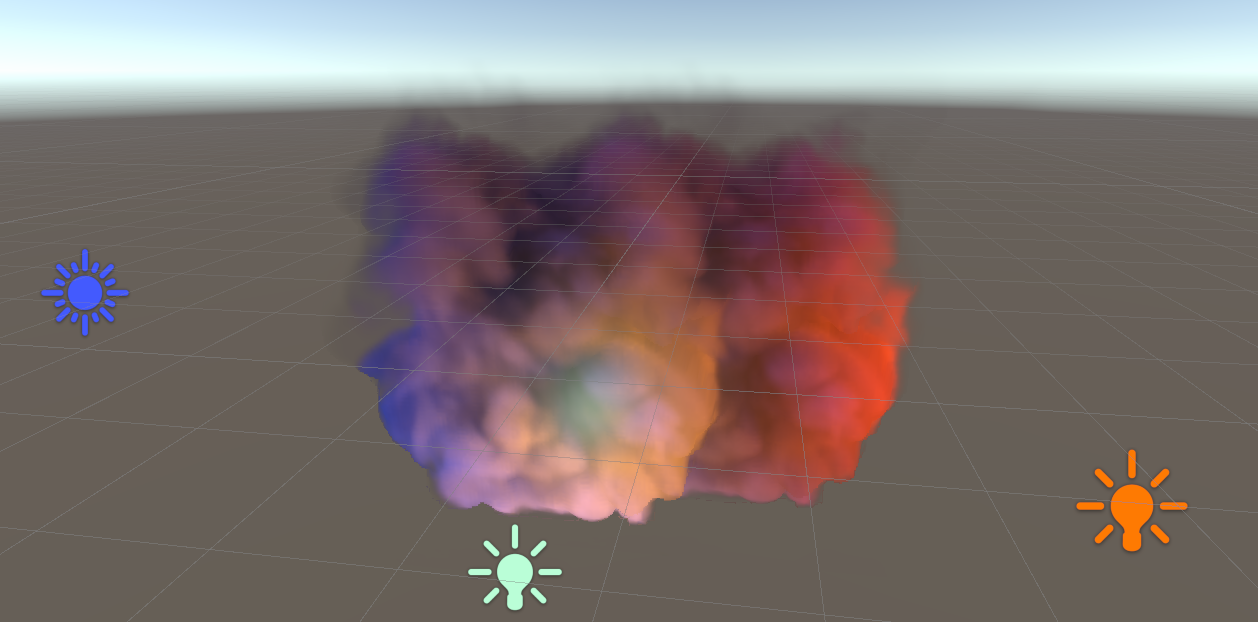
\includegraphics[width=0.89\textwidth]{Grafiken/Evaluation/pomShadows.png}
	\begin{footnotesize}
		\caption{Kein gegenseitiger Schattenwurf bei POM-basierten Billboards. }
		\label{fig:pomShadows}
	\end{footnotesize}
\end{figure}




%How, wie viele?

Ein weiterer Vorteil, der sich aus dieser Methode ergibt, sind die Texture Sheets. In eine einzige Textur lassen sich 4 verschiedene Informationen in die
RGBA-Kanäle speichern. Neben den verschiedenen Lightmaps aus 6 Richtungen können beispielsweise noch ein Color-Key oder Emission- und Heatmaps gespeichert werden.
Mit weiteren Infos wie einer Heatmap lässt sich ein Übergang, bzw. eine Mischung von Feuer und Rauch erzeugen. Dies ist ein Phänomen, welches sich bei größeren Bränden
oder Explosionen beobachten lässt (\textbf{\autoref{fig:explosion}}).
Die Anzahl der Lightmaps lässt sich auch reduzieren, indem die Lichtrichtungen von vorne und von hinten im Shader approximiert werden können.
Es gibt viele Möglichkeiten, die Flexibilität von Texturen ausnutzen zu können und dabei die Menge an benötigten Daten und Berechnungen gering zu halten,
sodass der flüssige Einsatz in VR gegeben bleibt. Weiterhin lassen sich auf Kosten weiterer Texture Sheets
verschiedene Simulationen erstellen, sodass größere Varianz in das Aussehen des Partikelsystems eingebracht werden kann.
Durch die unendliche Wiederholbarkeit kann die Animation ab einem zufällig gewählten Frame starten, wodurch schon mit einer einzigen Animation
kaum auffällt, dass das ganze System auf dieser einen Animation basiert.


Neben den ganzen Vorteilen, die diese Variante mit sich bringt gibt es auch negative Punkte. Bei zu geringer Auflösung sehen die Renderings schnell
verpixelt aus, je näher diese betrachtet werden. Dies ist ein großer Nachteil der Texture Sheets. Wird die Auflösung jedes Frames verdoppelt, also in diesem
Fall von 256x256 Pixeln auf 512x512 Pixel, so erhöht sich die Auflösung der gesamten Textur um den Faktor vier für jeden der RGBA-Kanäle. Selbst dann sind
die einzelnen Frames noch relativ gering aufgelöst und nicht für die Betrachtung aus der Nähe gedacht. Je detaillierter die Simulation auf denen die Texture Sheets basieren,
desto höher sollte die Auflösung sein um auch alle diese Details abbilden zu können.
Die visuellen Artefakte, wie beispielsweise das Einschneiden der benachbarten Frames aus dem Texture Sheet aus einem flachen Betrachtungswinkel (\textbf{\autoref{fig:smokeBleeding}}),
schränken die Einsatzmöglichkeiten für die Anwendung in VR stark ein.
Bei der Darstellung des Feuers kommt der Faktor hinzu, dass Billboards nicht als Lichtquelle fungieren, was dem Realismus der Simulation schadet.

Abschließend lässt sich zu dem Rendering von Feuer und Rauch auf Basis von Parallax Occlusion Mapping sagen, dass sich diese Variante, so wie sie für diese Arbet
implementiert ist, nicht immer eignet. Die visuellen Artefakte erzeugen Störungen der Immersion. Jedoch wird das Parallax Offset in der Stereoansicht korrekt dargestellt,
wodurch dieser Ansatz vielversprechend bleibt. Es ist wahrscheinlich, dass es für die genannten Probleme elegante Lösungen gibt, die in Zukunft an anderer Stelle 
betrachtet werden könnten.



CONTRA\newline
- Transparenz ist irgendwie weird\newline
- Geringe Auflösung der einzelnen Frames, doppelte Auflösung = 4fache Texturgröße \newline
% - Basiert immernoch auf Billboards\newline
%  -> Trotz simulierter Tiefe ein flacher Eindruck in VR\newline
- Funktioniert nicht gut bei mehreren Lichtquellen\newline
- Schattenwurf auf Umgebung funktioniert nicht\newline
- Beleuchtung der  Umgebung auch nicht möglich\newline

\begin{figure}[h!]
	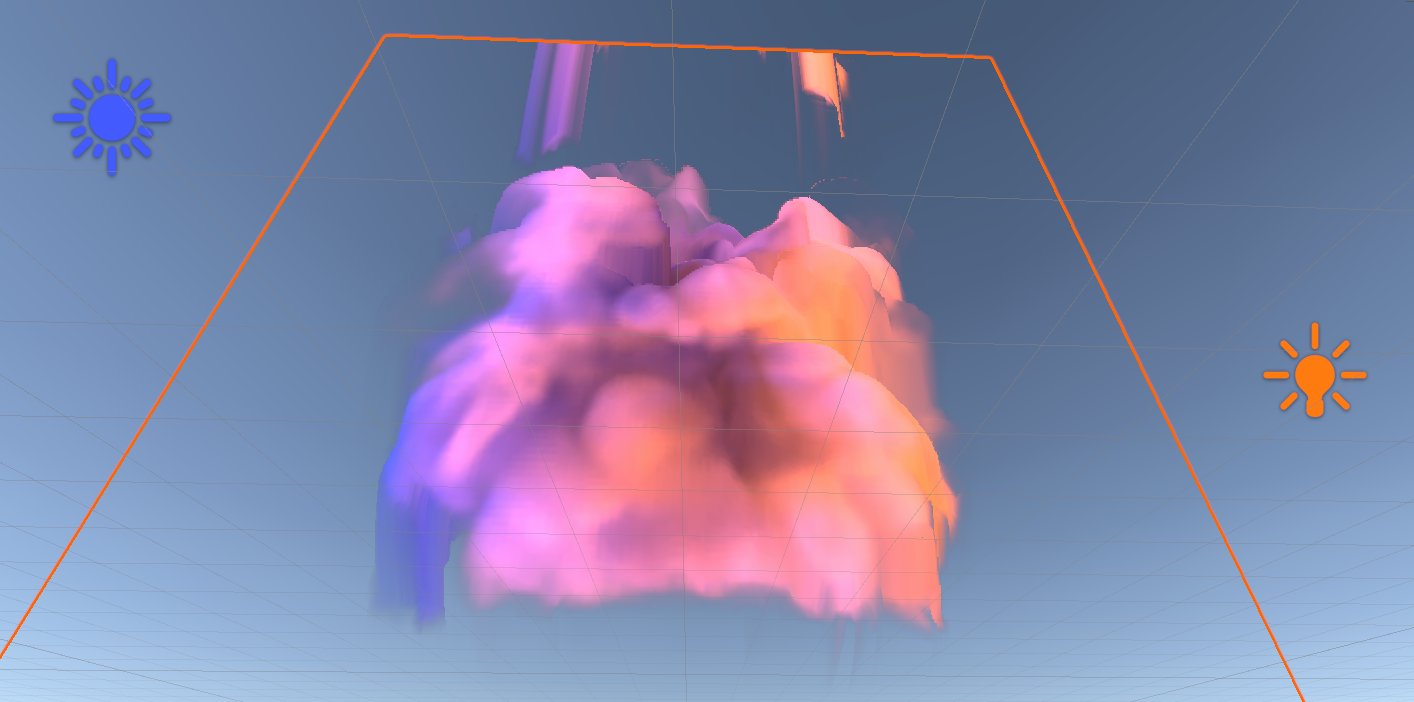
\includegraphics[width=0.89\textwidth]{Grafiken/Evaluation/Smoke_artefacts.png}
	\centering
	\begin{footnotesize}
		\caption{Verzerrungsartefakte bei der Anwendung von Parallax Occlusion Mapping mit zu starkem Offset. Die benachbarten Frames des Texture Sheets
			werden ebenfalls mit verzerrt, wodurch Fragmente davon, bei flachem Betrachtungswinkel, mit in das Billboard einlaufen.}
		\label{fig:smokeBleeding}
	\end{footnotesize}
\end{figure}



\subsection{Ray Marching}
\label{sec:5.2}

Aufgrund der massiven Einschränkungen in der Qualität des Exports aus Houdini wurde, für die bessere Betrachtung in VR, ein Set Volume Slices aus dem Github-Repository von Dylan Meville, 
verwendet\footnote{\url{https://github.com/DMeville/DMVolumeRendering/blob/main/DMVolumeRendering/Assets/VolumeRubberCube.exr}, abgerufen am 28.07.2022}.



PRO: \newline
- Sehr günstige AO aufgrund der bereits berechneten Distanz\newline
- Lichtstrahl in Volumen weiterverfolgen kann Schatten erzeugen\newline
-

CONTRA: \newline
- Aufwändigere Berechnung\newline
- 3D-Datenset beinhaltet keine Animation der Textur\newline




